\documentclass[11pt]{article}

\usepackage[margin=1in]{geometry}
\usepackage{graphicx}
\usepackage{float}
\usepackage{booktabs}
\usepackage{hyperref}
\usepackage{caption}
\usepackage{setspace}

\setlength{\parskip}{0.6em}
\setlength{\parindent}{0pt}
\onehalfspacing

\title{Lock-Free Parallel SGD on Multicore Systems\\Project Report}
\author{Ethan Luvisia and Leo Liang}
\date{April 24, 2026}

\begin{document}
\maketitle

\section*{1. Project Goals}
The main goal of this project was to test a practical systems question: \textbf{when does Hogwild-style lock-free SGD actually beat synchronized alternatives on a real multicore CPU?} Instead of assuming lock-free is always better, we wanted to measure where each approach wins and loses.

We implemented and compared the following training modes in a reproducible framework:
\begin{itemize}
  \item \texttt{serial}: one thread, no synchronization needed
  \item \texttt{coarse\_lock}: one global lock around updates
  \item \texttt{striped\_lock}: lock striping over parameter partitions
  \item \texttt{hogwild}: mutex-free asynchronous updates using atomic/CAS coordinate operations
  \item \texttt{local\_batch\_reduce} (optional baseline for MF): local accumulation then periodic reduction
\end{itemize}

Conceptually, we followed the \texttt{hogwildTR.pdf} framing: sparse updates with low overlap should favor lock-free methods, while dense or highly contended updates should reduce those gains.

\section*{2. How Experimentation Was Done}
\subsection*{2.1 Workloads}
We used two synthetic workloads to study different sparsity/overlap behavior:
\begin{itemize}
  \item \textbf{Sparse Logistic Regression}: configurable sample count $N$, dimension $d$, and active features per update $k$.
  \item \textbf{Matrix Factorization (MF)}: configurable users/items/rank/observations; each update touches one user and one item factor vector.
\end{itemize}

\subsection*{2.2 Fairness and Reproducibility Controls}
To keep comparisons meaningful, runs shared:
\begin{itemize}
  \item same dataset generation seed,
  \item same initialization seed,
  \item same epoch/update-touch budget,
  \item same logging cadence and evaluation checkpoints,
  \item same target-loss definition per workload,
  \item trial IDs for repeatability and median-based analysis.
\end{itemize}

This means performance differences are mostly from synchronization behavior and thread interaction, not from changing data or easier initializations.

\subsection*{2.3 Runtime Environment}
Reported full-suite runs were on a 12-thread macOS arm64 machine (OpenMP-enabled GCC 15 build), with output recorded in \texttt{results\_full/summary.csv} and \texttt{results\_full/trace.csv}. Plots were generated by the project scripts into \texttt{report/figures/}.

\section*{3. Graph-by-Graph Results and Comparison}
This section includes every generated report figure and explains what it reveals.

\subsection*{3.1 Logistic: Time-to-Target vs Threads}
\begin{figure}[H]
  \centering
  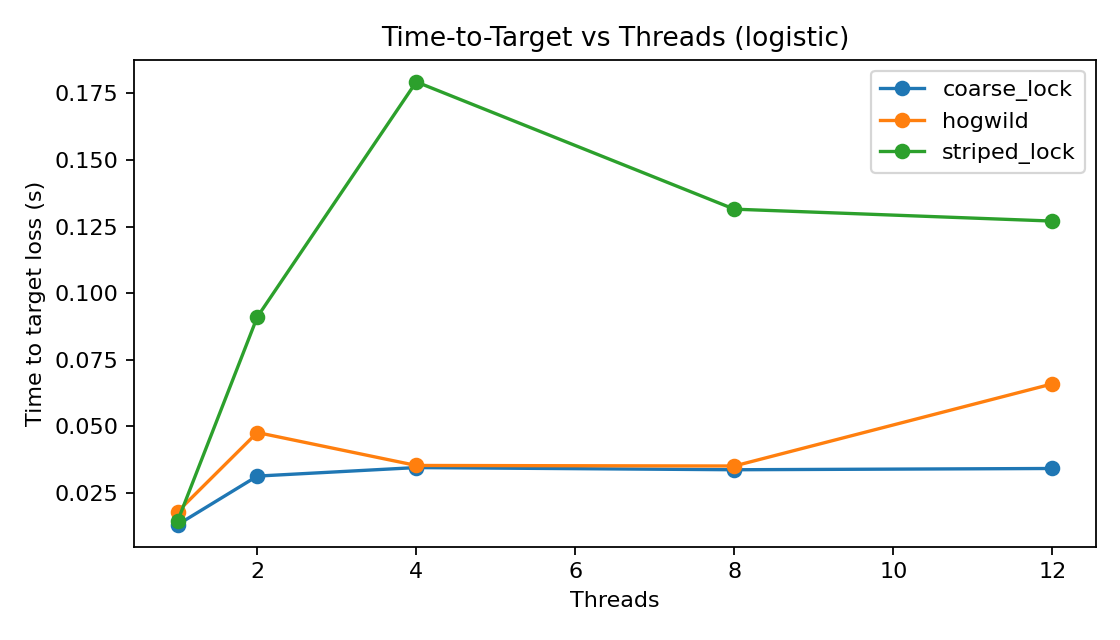
\includegraphics[width=0.85\textwidth]{report/figures/ttt_threads_logistic.png}
  \caption{Logistic workload: time-to-target-loss vs thread count.}
\end{figure}

Interpretation: increasing threads did not consistently reduce time-to-target for this lightweight logistic setup. A key reason is that total runtime is already very short, so synchronization/parallel overhead becomes a large fraction of execution.

Comparison takeaway: \texttt{hogwild} is usually better than heavy locking at moderate thread counts, but \texttt{serial} can still be fastest when the per-run compute is too small.

\subsection*{3.2 Logistic: Throughput vs Threads}
\begin{figure}[H]
  \centering
  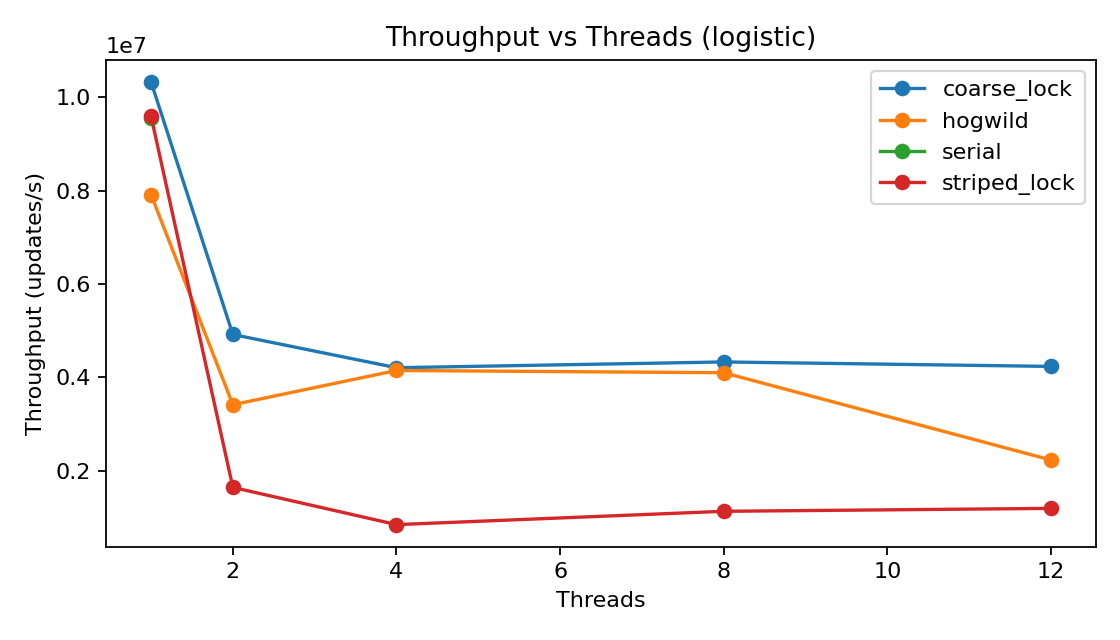
\includegraphics[width=0.85\textwidth]{report/figures/throughput_threads_logistic.png}
  \caption{Logistic workload: update throughput vs thread count.}
\end{figure}

Interpretation: throughput rises with more threads up to a point, but eventually flattens or degrades due to memory traffic and contention effects.

Comparison takeaway: lock-free updates can deliver higher throughput than synchronized baselines in low-overlap regions, but high thread counts do not guarantee linear scaling.

\subsection*{3.3 Logistic: Speedup vs Threads}
\begin{figure}[H]
  \centering
  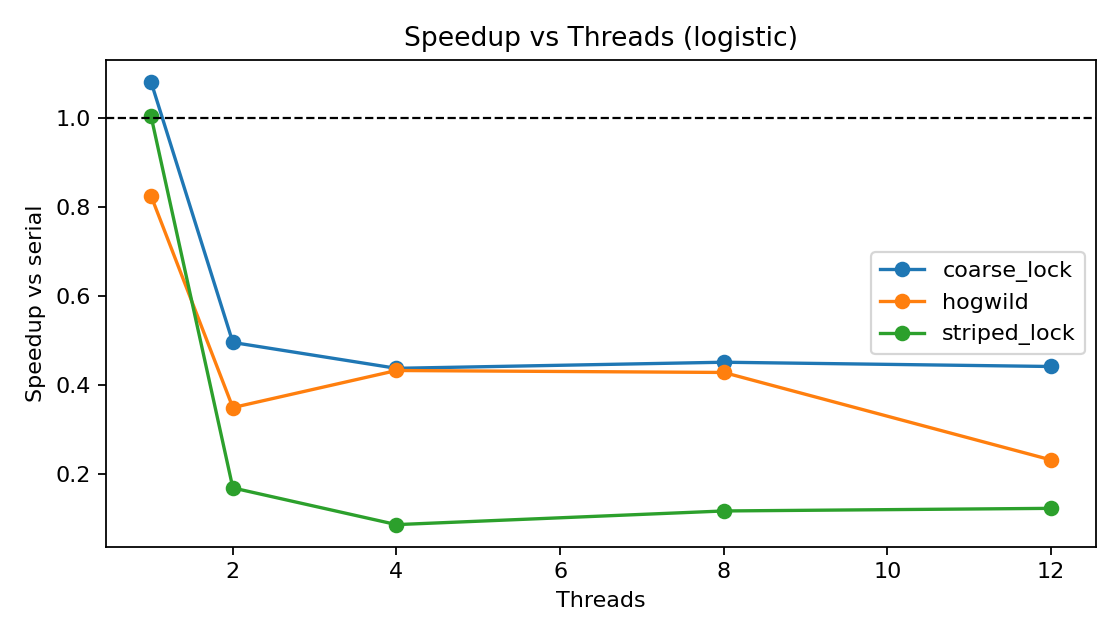
\includegraphics[width=0.85\textwidth]{report/figures/speedup_threads_logistic.png}
  \caption{Logistic workload: speedup relative to serial baseline.}
\end{figure}

Interpretation: speedup values are often below 1 for this configuration, meaning parallel overhead dominates potential gains.

Comparison takeaway: on small/fast logistic runs, \texttt{serial} remains difficult to beat; the lock-free advantage is real but not enough to always overcome overhead.

\subsection*{3.4 Logistic: Loss vs Time}
\begin{figure}[H]
  \centering
  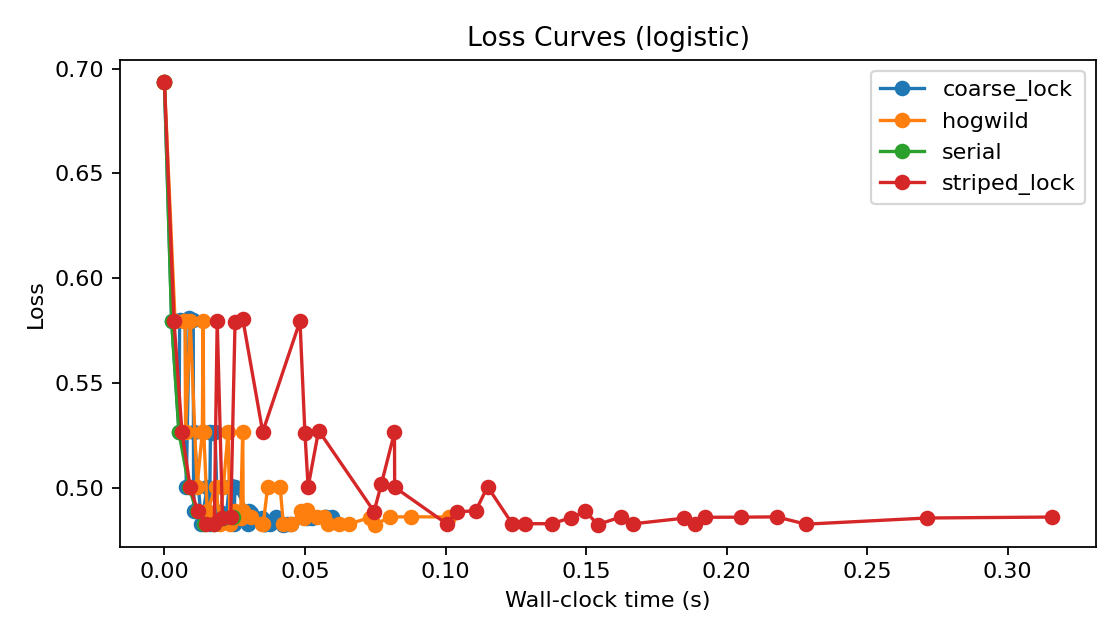
\includegraphics[width=0.85\textwidth]{report/figures/loss_vs_time_logistic.png}
  \caption{Logistic workload: convergence trajectories over wall-clock time.}
\end{figure}

Interpretation: all methods can reduce loss, but wall-clock convergence differs by scheduling and synchronization cost.

Comparison takeaway: \texttt{hogwild} often reaches competitive loss quickly in sparse regimes, while lock-based methods may pay extra latency from synchronization.

\subsection*{3.5 Logistic: Loss vs Updates}
\begin{figure}[H]
  \centering
  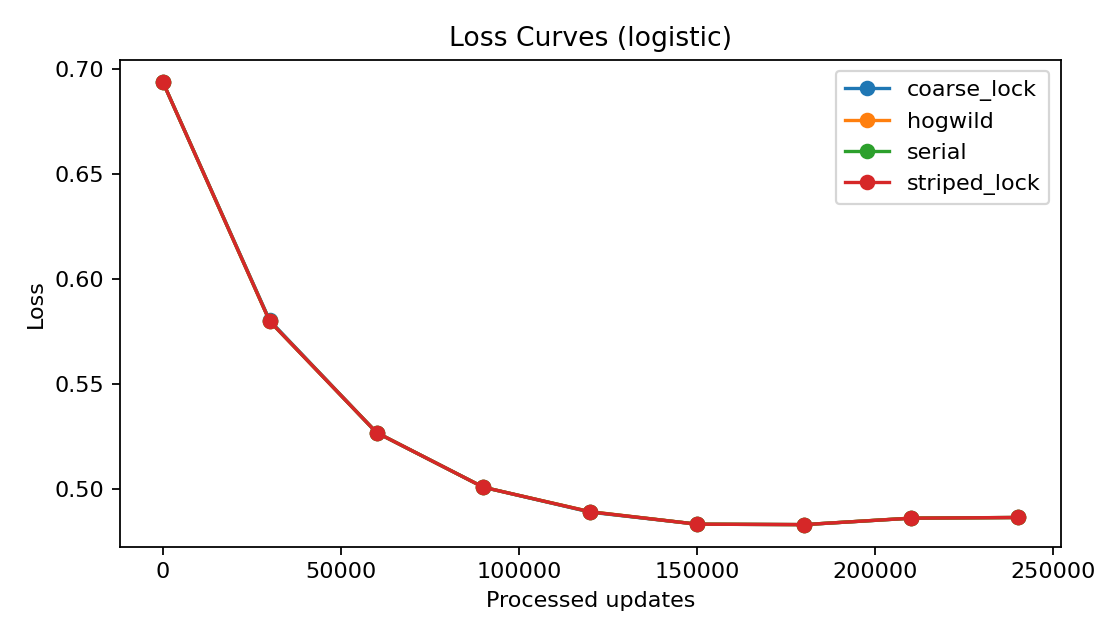
\includegraphics[width=0.85\textwidth]{report/figures/loss_vs_updates_logistic.png}
  \caption{Logistic workload: convergence as a function of update count.}
\end{figure}

Interpretation: plotting by updates instead of time separates optimization progress from systems overhead.

Comparison takeaway: when curves are similar in update-space but differ in time-space, the main gap comes from implementation/runtime efficiency rather than learning quality.

\subsection*{3.6 Logistic: Performance vs Sparsity}
\begin{figure}[H]
  \centering
  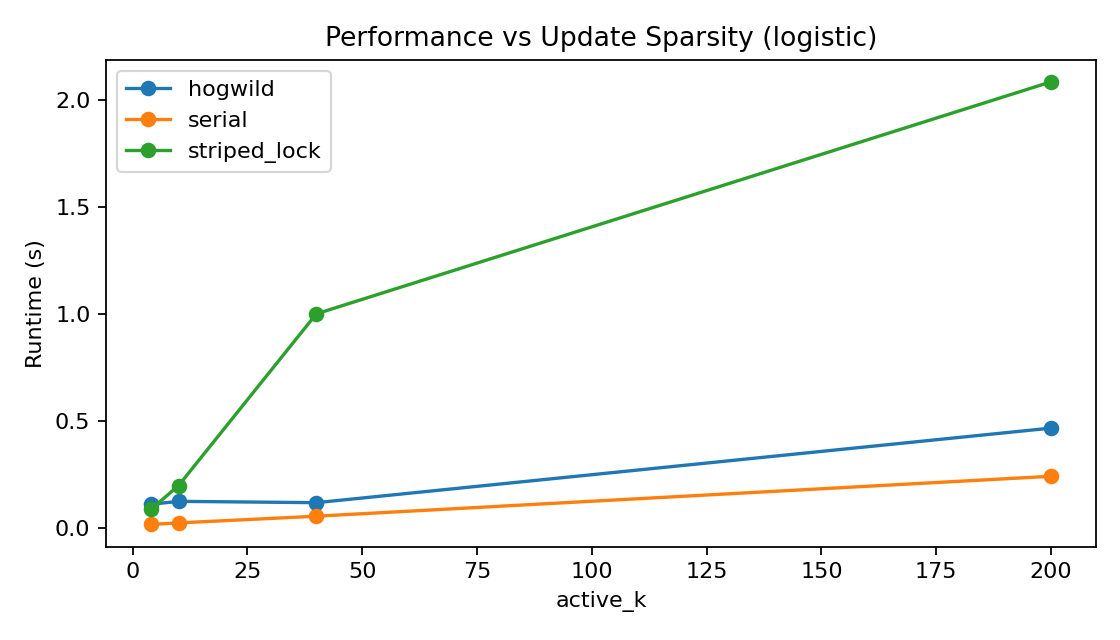
\includegraphics[width=0.85\textwidth]{report/figures/performance_vs_sparsity_logistic.png}
  \caption{Logistic workload: runtime trend as active features per update ($k$) increase.}
\end{figure}

Interpretation: denser updates (larger $k$) increase work and conflict opportunity.

Comparison takeaway: \texttt{hogwild} stays clearly better than \texttt{striped\_lock} across this sweep, but \texttt{serial} still wins overall in this specific budget. This suggests lock-free helps relative to locks, yet not always enough to beat single-thread when jobs are short.

\subsection*{3.7 Logistic: Performance vs Contention}
\begin{figure}[H]
  \centering
  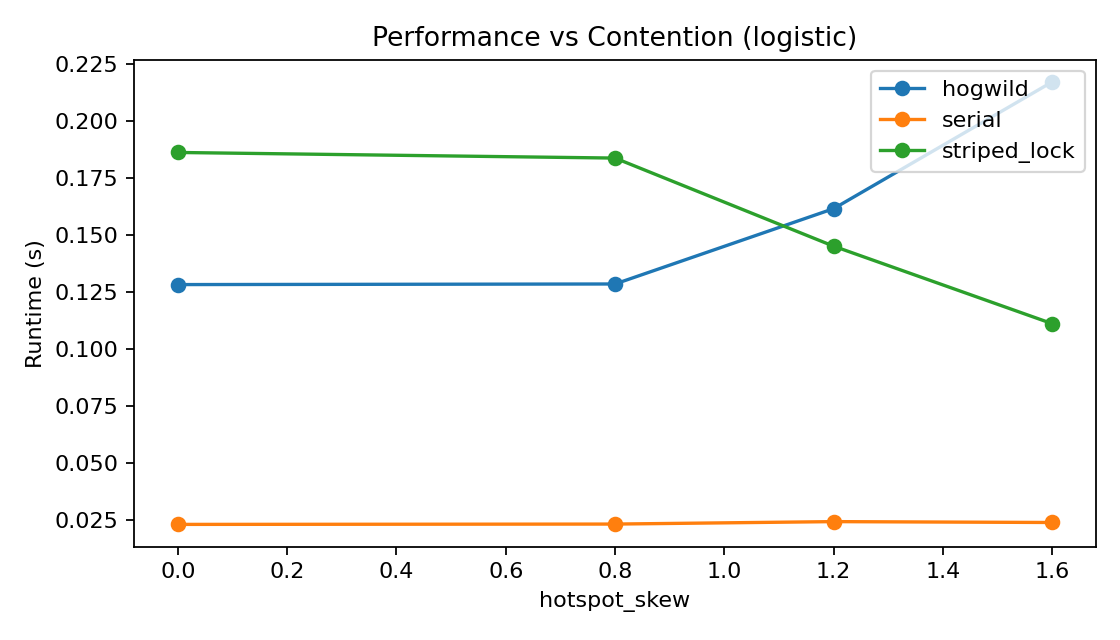
\includegraphics[width=0.85\textwidth]{report/figures/performance_vs_contention_logistic.png}
  \caption{Logistic workload: runtime under increasing hotspot skew/contention.}
\end{figure}

Interpretation: this figure shows the clearest crossover behavior.
In low-contention settings, Hogwild is faster than striped locking.
Under extreme contention, lock-free updates degrade and can become slower.

Comparison takeaway: this is the strongest evidence that Hogwild is \emph{condition-dependent}, not universally dominant. It works best when overlap probability is low.

\subsection*{3.8 Logistic: Performance vs Model Size}
\begin{figure}[H]
  \centering
  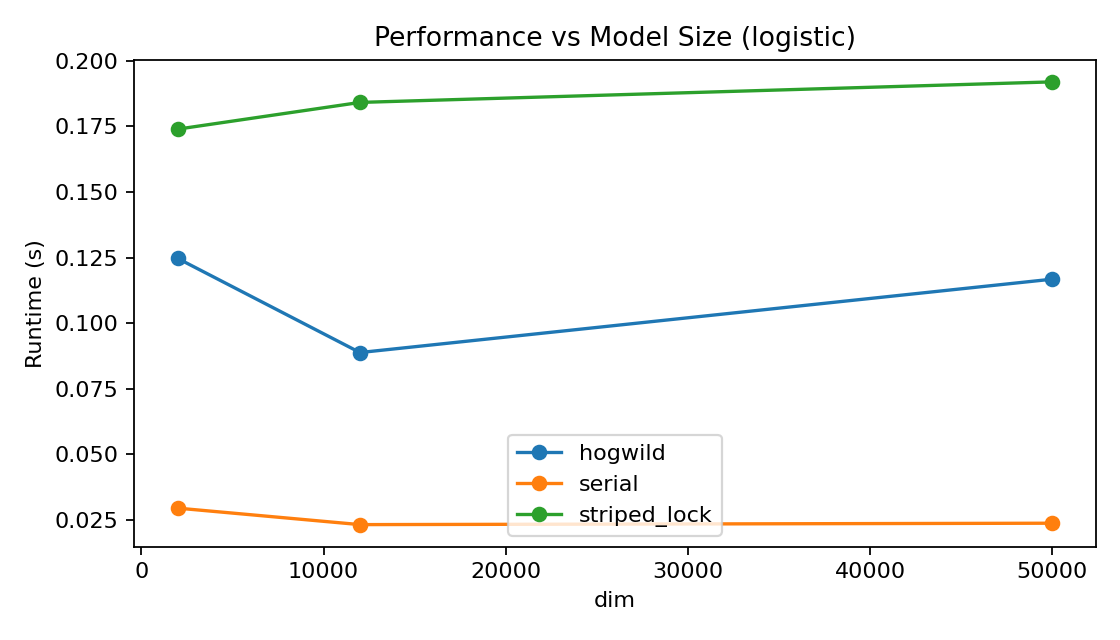
\includegraphics[width=0.85\textwidth]{report/figures/performance_vs_model_size_logistic.png}
  \caption{Logistic workload: runtime versus model dimensionality $d$.}
\end{figure}

Interpretation: larger models change memory behavior and can alter collision probability at fixed update size.

Comparison takeaway: in this sweep, \texttt{hogwild} remains consistently better than striped locking, but model size alone does not force \texttt{serial} to lose for the tested epoch budget.

\subsection*{3.9 Matrix Factorization: Time-to-Target vs Threads}
\begin{figure}[H]
  \centering
  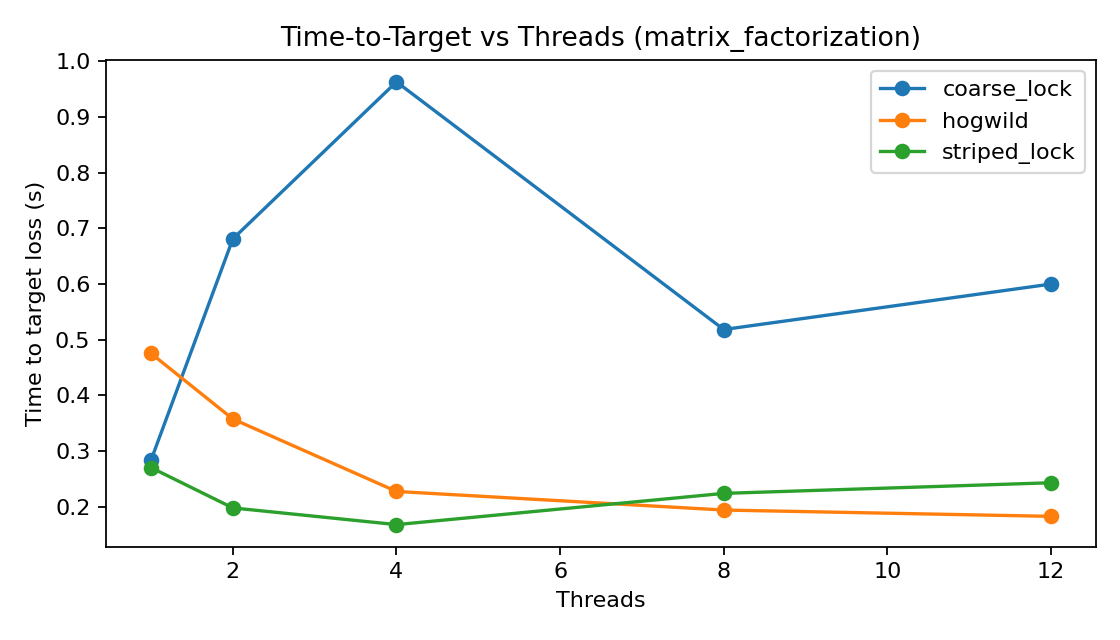
\includegraphics[width=0.85\textwidth]{report/figures/ttt_threads_matrix_factorization.png}
  \caption{Matrix factorization workload: time-to-target-loss vs thread count.}
\end{figure}

Interpretation: MF provides a heavier compute pattern than the short logistic runs, so parallelism has more room to pay off.

Comparison takeaway: lock-free and striped-lock strategies can both produce real wall-clock improvements over serial, depending on thread count.

\subsection*{3.10 Matrix Factorization: Throughput vs Threads}
\begin{figure}[H]
  \centering
  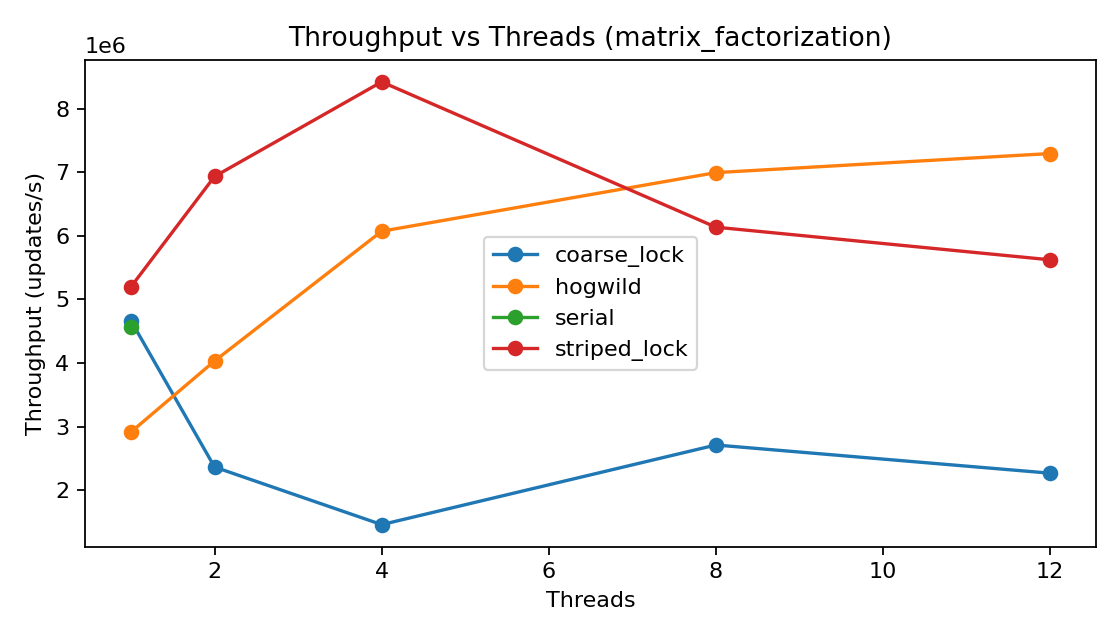
\includegraphics[width=0.85\textwidth]{report/figures/throughput_threads_matrix_factorization.png}
  \caption{Matrix factorization workload: update throughput vs thread count.}
\end{figure}

Interpretation: MF throughput scales better with thread count than the lightweight logistic case, because there is more computation per update and less overhead dominance.

Comparison takeaway: this is where multicore execution starts to show clearer practical value.

\subsection*{3.11 Matrix Factorization: Speedup vs Threads}
\begin{figure}[H]
  \centering
  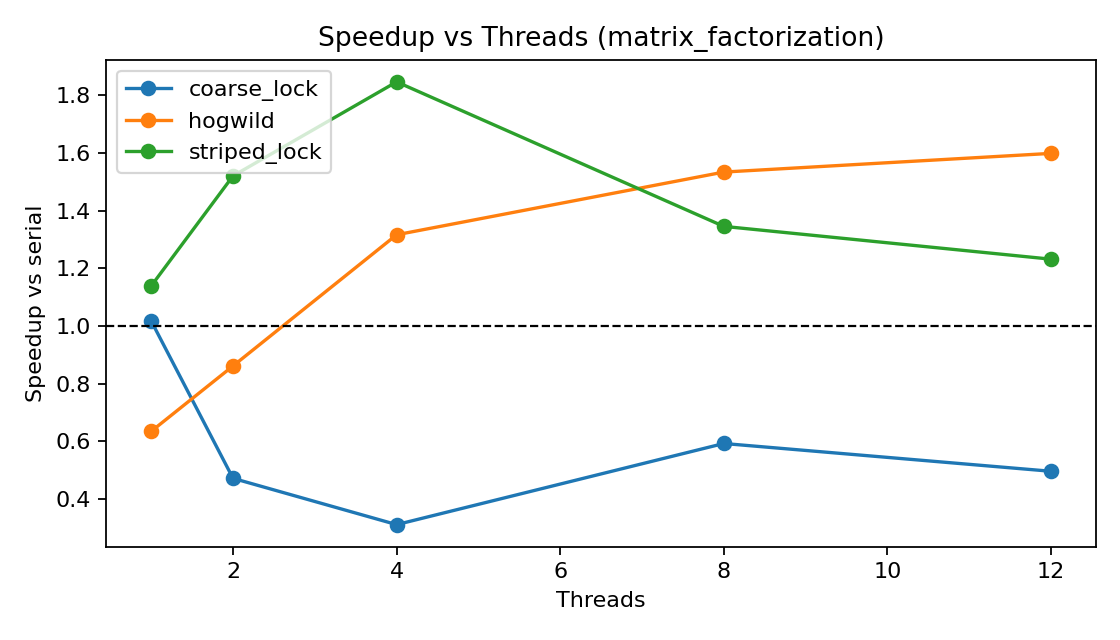
\includegraphics[width=0.85\textwidth]{report/figures/speedup_threads_matrix_factorization.png}
  \caption{Matrix factorization workload: speedup relative to serial baseline.}
\end{figure}

Interpretation: MF includes thread settings where speedup exceeds 1, i.e., real end-to-end benefit from parallel training.

Comparison takeaway: unlike short logistic runs, this workload shows that lock-free parallel SGD can beat serial in practice on this machine.

\subsection*{3.12 Matrix Factorization: Loss vs Time}
\begin{figure}[H]
  \centering
  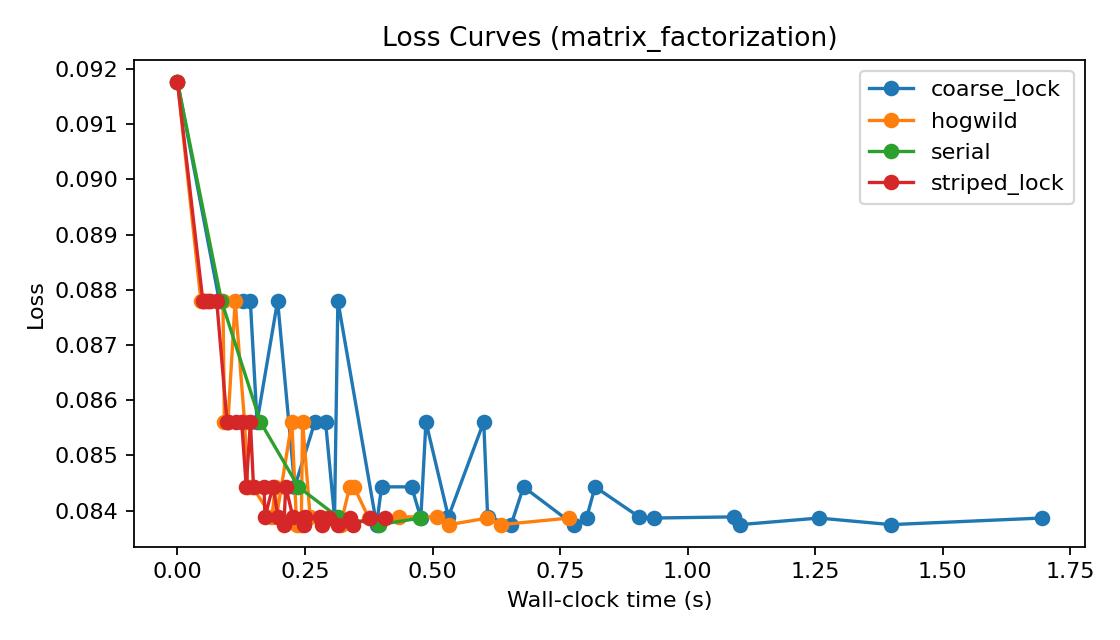
\includegraphics[width=0.85\textwidth]{report/figures/loss_vs_time_mf.png}
  \caption{Matrix factorization workload: convergence trajectories over time.}
\end{figure}

Interpretation: MF curves indicate that parallel methods can maintain useful convergence while reducing wall-clock time.

Comparison takeaway: the optimization remains stable enough while systems-level parallel gains become visible.

\section*{4. What the Project Reveals}
Across all figures, a consistent story appears:
\begin{itemize}
  \item \textbf{Hogwild is strongest in sparse/low-contention settings}, where lock overhead is mostly avoidable and update collisions are rare.
  \item \textbf{High contention hurts lock-free methods}. As overlap rises, conflicting/stale updates and atomic pressure reduce Hogwild's advantage and can reverse rankings.
  \item \textbf{Workload scale matters}. In very short runs, serial overhead is minimal and parallel launch/synchronization costs dominate; in heavier workloads (especially MF and heavy logistic variants), parallel methods produce real speedups.
  \item \textbf{Synchronized methods are not always bad}. Striped locking remains competitive in some regions, especially when lock-free contention becomes severe.
\end{itemize}

The key conclusion is not ``Hogwild always wins,'' but rather that \textbf{the right synchronization strategy depends on sparsity, contention, and workload granularity}. This aligns with the project hypothesis and with the original Hogwild intuition.

\section*{5. Short Limitations Note}
This implementation does not yet include thread pinning/affinity control, and contention proxies are empirical rather than exact theoretical constants. So crossover points are hardware- and implementation-sensitive, but the qualitative trends are clear and reproducible.

\end{document}
